\documentclass[letterpaper]{article}
\usepackage[submission]{aaai2027}
\usepackage[hyphens]{url}
\usepackage{graphicx}
\usepackage{tikz}
\usetikzlibrary{arrows.meta, positioning, fit, calc, shapes.geometric}
\usepackage{microtype}
\usepackage{natbib}
\urlstyle{rm}
\def\UrlFont{\rm}
\usepackage{caption}
\frenchspacing
\usepackage{amsmath}
\usepackage{amssymb}
\usepackage{booktabs}
\usepackage{multirow}
\usepackage{cuted}
\emergencystretch=1.2em
\pdfinfo{
/TemplateVersion (2027.1)
}
\setcounter{secnumdepth}{0}

\title{WEAVE: Overcoming the Identity Shortcut in Style Transfer via 3-Minute Wavelet-Decoupled Flow Matching}
\author{Anonymous Submission}
\affiliations{}
\begin{document}
\maketitle

\begin{abstract}
Current style transfer methods face two primary challenges. First, state-of-the-art diffusion models, along with training-free methods built on them, require more than 60\,GB of VRAM and therefore cannot run on consumer GPUs. Second, lightweight methods without these generative backbones often underperform a trivial identity mapping, which scores high on traditional metrics like ArtFID and LPIPS but was rarely evaluated as a baseline. 

We empirically observe that frequency dominance in shared representation spaces pushes lightweight models toward identity-like solutions~\cite{rahaman2019spectral}: low-frequency structural energy overwhelms high-frequency style gradients, a pattern we confirm through gradient-spectrum analysis and per-subband style-transfer measurements.

We argue that an effective style transfer method should outperform the identity baseline while remaining computationally affordable. To this end, we propose WEAVE: a single-level Haar wavelet transform splits the VAE latent into a low-frequency structure band and high-frequency style bands; a compact rectified-flow network learns a structure-preserving velocity field; and endpoint statistical alignment (AdaIN) injects the target style into the high-frequency subbands. This decoupling separates content transport from style injection, letting WEAVE train in 3 minutes on a single consumer GPU.

We also advocate the IDT--TGT sandwich as an intuitive evaluation guideline. IDT returns the source unchanged, while TGT returns an unrelated image from the target style; together they show whether an output gains style without giving up source content beyond the target-reference level. Under this guideline, WEAVE clears the identity reference with only 903K trainable parameters (plus a frozen 84M VAE), making high-quality style transfer both effective and affordable.

\end{abstract}

\begin{strip}
\noindent
\includegraphics[width=\textwidth]{fig_distinct5_page1_summary.pdf}
\captionof{figure}{IDT--TGT sandwich comparison on Distinct5-WikiArt.
Left: style affinity $\frac{1}{2}(\mathrm{DINO\text{-}S}+\mathrm{CLIP\text{-}S})$ versus $1-\mathrm{LPIPS}$, with bubble area encoding training time.
The red points mark two WEAVE operating points.
Square markers denote training-free diffusion editors (StyleAligned).
The dashed line marks the IDT style reference (0.556); methods below it have not moved in the requested direction.
The dotted line marks the TGT content reference (0.267); methods right of it are perceptually farther from the source than an unrelated target-style image.
Right: target-pooled ArtFID on the same benchmark, with numbers inside the bars indicating training or response time.}
\label{fig:page1}
\end{strip}

\section{Introduction}

Style transfer faces a practical tension. Large diffusion editors can require more than 60\,GB of GPU memory, while lightweight models may preserve the source so strongly that their style score falls below the unchanged input. Metrics such as LPIPS and ArtFID can hide this no-op behavior because they reward source reconstruction and rarely report identity as a baseline.
Figure~\ref{fig:page1} adds two simple references. Identity (IDT) returns the source image, and Target Style (TGT) returns an unrelated reference from the requested style. A useful method should move beyond IDT in style without moving as far from the source as TGT. We offer this bracket as a diagnostic addition to existing metrics: it makes style suppression and content loss easier to read without replacing standard evaluation or judging a method outside this setting.

We trace the identity shortcut to frequency dominance rather than model size. Neural networks fit low-frequency signals first~\cite{rahaman2019spectral,xu2022frequency}, and natural images place much more energy in global structure than in fine texture. When flow matching learns both in one coordinate system, structural errors dominate the update and weaken the style-conditioned signal, a conflict also observed in frequency-domain translation~\cite{cai2021fdit}.

To solve the conflict between structure and style, we propose WEAVE.
WEAVE keeps the pre-trained VAE but replaces the diffusion network with a 903K-parameter velocity model. A one-level Haar transform separates low-frequency structure (LL) from high-frequency texture (LH/HL/HH). The flow learns content-preserving transport, and one endpoint AdaIN update injects style into the high-frequency bands. WEAVE trains in 3 minutes on one consumer GPU, and the same latent operation can be added to a frozen SD1.5 pipeline without training (Section~\ref{sec:plugin}).

\paragraph{Contributions.}
(1)~\textbf{Evaluation:} We advocate the IDT--TGT sandwich, an intuitive guideline that reports a no-op reference and a target-style reference alongside existing metrics.
(2)~\textbf{Method:} WEAVE separates structure and texture with Haar wavelets, then combines compact flow matching with endpoint high-frequency AdaIN.
(3)~\textbf{Efficiency:} WEAVE uses 903K trainable parameters, trains in 3 minutes on one RTX~3060, and transfers its latent operator to frozen SD1.5 without training.

\section{Related Work}
\label{sec:related}

\subsection{Neural Style Transfer}
\label{sec:rw-nst}
Artistic style transfer was introduced by optimizing pixels to match feature statistics of a pretrained network~\cite{gatys2015neural,gatys2016image}. AdaIN~\cite{huang2017arbitrary} and whitening--coloring transforms (WCT)~\cite{li2017universal} made this alignment feed-forward. GAN- and contrastive-learning approaches later addressed unpaired translation, notably CUT~\cite{park2020cut}, while feed-forward and attention-based variants improved correspondence and fidelity~\cite{park2019sanet,deng2022stytr2,hong2023aespa,kwon2024aesfa}. Training-free methods reuse pretrained codebooks or vision transformers~\cite{gim2024cast,zhang2024s2wat}. These lines improve flexibility, but content and style still interact in a shared feature space, where stronger style often changes source structure.

\subsection{Diffusion-based and Training-free Style Editing}
\label{sec:rw-diffusion}
Latent diffusion models~\cite{rombach2022high} move editing into a compressed generative space. Attention control and inversion support training-free manipulation~\cite{hertz2022prompt,meng2021sdedit}; StyleID and StyleAligned modify attention statistics~\cite{chung2024style,hertz2024style}; and IP-Adapter, InST, DiffuseIT, ArtBank, and Z-STAR broaden image-conditioned or inversion-based transfer~\cite{ye2023ipadapter,zhang2023inst,kim2022diffuseit,zhang2024artbank,lu2024zstar}. These methods benefit from strong priors, but recent backbones such as FLUX and Qwen-Image remain costly on consumer hardware~\cite{blackforestlabs2024flux,alibaba2024qwen}. WEAVE instead asks how much of the transfer can be learned after the representation and endpoint operation are fixed.

\subsection{Flow Matching and Schr\"odinger Bridges}
\label{sec:rw-sb}
Rectified flow~\cite{liu2022rectified} and flow matching~\cite{lipman2022flow} learn short transport paths with few integration steps. Schr\"odinger bridges~\cite{leonard2014survey} and their diffusion or flow solvers---DSB, DSBM, I2SB, and DDIB~\cite{debortoli2021dsb,shi2023dsbm,liu2023i2sb,su2023ddib}---extend transport to unpaired distributions. Most operate in one coordinate basis, so errors from content geometry and style appearance compete in the same regression. WEAVE retains the short-path advantage but changes the coordinates and target before learning the velocity.

\subsection{Lightweight Models and Evaluation}
\label{sec:rw-light}
Mamba-based SaMST and SaMam reduce the trainable model size~\cite{liu2024samst,liu2024samam,gu2023mamba}. However, common measures such as LPIPS~\cite{zhang2018unreasonable} and ArtFID~\cite{wright2022artfid} strongly reward source reconstruction. Reporting only these scores can make a weakly stylized output look favorable. Our IDT--TGT protocol therefore adds the unchanged source and a source-independent target-style image as empirical references. It keeps the original metrics, but makes both insufficient style movement and excessive content loss visible.

\subsection{Spectral Bias and Frequency-aware Optimization}
\label{sec:rw-spectral}
Neural networks preferentially fit low-frequency signals~\cite{rahaman2019spectral,xu2022frequency}, while natural images place most energy in coarse structure. Frequency-domain translation has used low-/high-frequency constraints to protect content identity~\cite{cai2021fdit}. Our probes connect this imbalance to the identity shortcut in lightweight style transfer: when one loss handles both structure and texture, the larger low-frequency residual dominates the update. This observation motivates separating the two before optimization.

\subsection{Wavelet and Latent-space Alignment}
\label{sec:rw-wavelet}
Wavelets separate local information by scale and orientation, and have been used in restoration, generation, and style transfer~\cite{phung2023wavelet,yoo2019photorealistic}. The Haar basis is orthogonal and admits exact reconstruction~\cite{daubechies1992ten}. Meanwhile, VAE latents provide a compact space in which statistical transforms such as AdaIN and WCT are inexpensive. WEAVE combines these ingredients inside flow matching: the wavelet basis separates the transport targets, and endpoint alignment supplies style statistics once the learned path is complete.



\section{Method}
\label{sec:method}

The difficult part of lightweight style transfer is not only model capacity. A direct
content-to-style target changes layout, palette, and texture at once. In latent MSE, the
large low-frequency structural residual dominates the smaller style residuals, so a compact
model can reduce its loss by staying close to the source. Increasing style strength inside
the same coordinates then tends to spend content instead of resolving the conflict.

WEAVE changes the problem before increasing the model. It constructs a source-aligned
training endpoint, expresses the transport in orthogonal Haar bands, and applies a single
high-frequency statistics update after the learned path. Figure~\ref{fig:framework}
summarizes these three stages.

\begin{figure*}[t!]
\centering
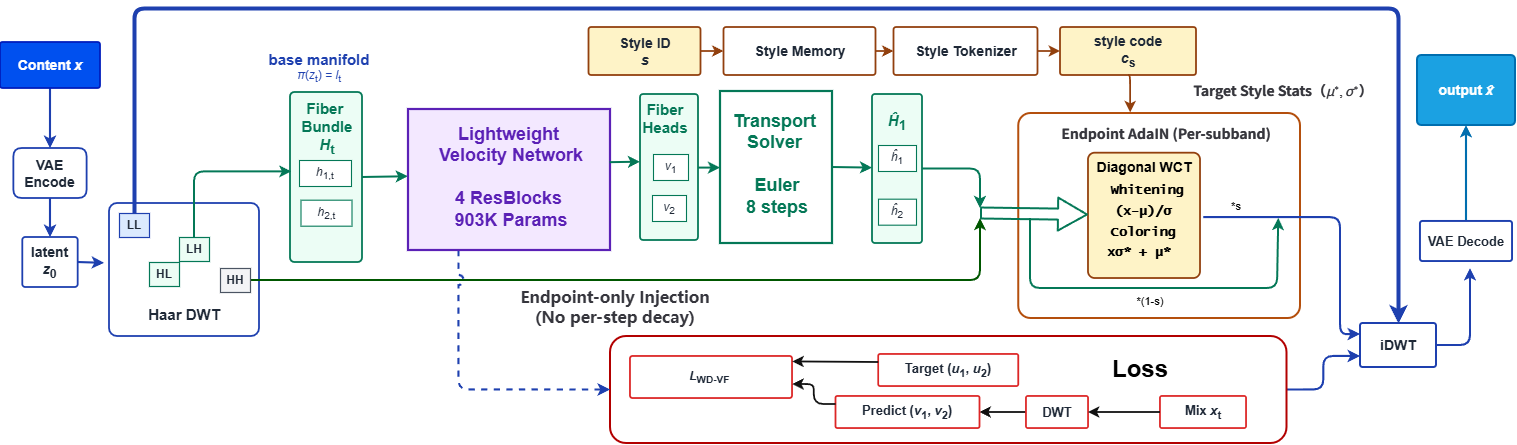
\includegraphics[width=\textwidth]{aaai_arch_diagram_v16_staggered_bundle.drawio.png}
\caption{\textbf{WEAVE architecture}. A single-level Haar transform exposes the LL/LH/HL/HH subbands of the SD1.5 VAE latent. The compact velocity network $v_\theta$ ($\sim$903K) predicts motion for LL/LH/HL via three heads, while HH carries no head. Band-weighted rectified-flow matching learns the transport; per-subband AdaIN aligns LH/HL/HH once at the endpoint with scales $0.3/0.3/0.5$ and leaves LL unchanged.}
\label{fig:framework}
\end{figure*}



\subsection{Framework Setup}
\label{sec:framework}

Let $z_c=\mathcal E(x_c)\in\mathbb R^{4\times32\times32}$ and
$z_s=\mathcal E(x_s)$ be content and target-style latents from the frozen SD1.5
VAE~\cite{rombach2022high}. A direct path from $z_c$ to $z_s$ also learns the unrelated
geometry of $x_s$. We instead decompose
$\mathcal W(z_c)=(\ell_c,h_{1,c},h_{2,c},h_{3,c})$ and similarly for $z_s$, then form
the structure-aligned endpoint
\begin{equation}
\begin{aligned}
\tilde\ell_s &=(1-\alpha)\ell_c+
\alpha\,\mathrm{AdaIN}(\ell_c,\ell_s),\qquad \alpha=0.3,\\
z_1^\star&=\mathcal W^{-1}(\tilde\ell_s,h_{1,s},h_{2,s},h_{3,s}).
\end{aligned}
\label{eq:aligned-target}
\end{equation}
The LL blend permits a mild palette and contrast change while keeping source layout. The
high-frequency target comes from the requested style. This target is important: using the
original source LL exactly suppresses coarse appearance, while using the complete style
latent asks the network to reproduce target-image geometry.

Rectified flow learns the straight path
\begin{equation}
z_t=(1-t)z_c+t z_1^\star,\qquad
u=z_1^\star-z_c,qquad t\sim\mathcal U([0,1]).
\label{eq:rf-path}
\end{equation}
Because $\mathcal W$ is linear, the same interpolation holds independently in every
subband. WEAVE therefore keeps the standard rectified-flow target and changes only the
endpoint, parameter sharing, and loss weights.

\subsection{Wavelet Decomposition and Frequency Routing}
\label{sec:wavelet}

Low-frequency structure carries much more energy than fine texture, so a shared loss favors source reconstruction~\cite{rahaman2019spectral,xu2022frequency,cai2021fdit}. WEAVE separates these signals before predicting the flow.

\paragraph{Haar wavelet decomposition.}
A one-level Haar transform gives $\mathcal W(z_t)=(\ell_t,h_{1,t},h_{2,t},h_{3,t})$: one LL structure band and three high-frequency bands, each $4{\times}16{\times}16$. Haar is orthogonal and local, so high-frequency updates do not directly alter the LL coordinate~\cite{daubechies1992ten}.
\begin{equation}
\|\Delta z\|_F^2=\|\Delta\ell\|_F^2+
\sum_{i=1}^{3}\|\Delta h_i\|_F^2.
\label{eq:haar-energy}
\end{equation}
Equation~\ref{eq:haar-energy} is simply Parseval's identity. It makes the design
transparent: an operation restricted to LH/HL/HH leaves the LL coefficient unchanged,
although the nonlinear VAE decoder can still couple visible color and texture.

\paragraph{Empirical frequency probes.}
Across 5,000 cross-style latent pairs, transport energy concentrates in LL while style separation is strongest in HH (Figure~\ref{fig:frequency-probes}). This motivates a weak LL loss and stronger high-frequency routing.

\begin{figure}[t]
\centering
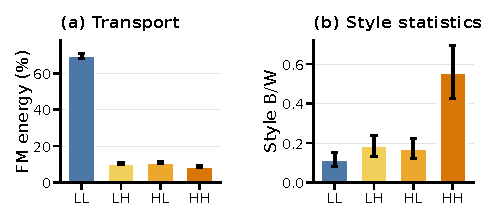
\includegraphics[width=0.98\columnwidth]{fig_probe_combined.pdf}
\caption{\textbf{Frequency probes.} (a) Cross-style transport energy in each Haar band. (b) Between-style versus within-style separation of latent statistics. Error bars summarize variation across style routes or statistics.}
\label{fig:frequency-probes}
\end{figure}

\begin{figure*}[t!]
\centering

\includegraphics[width=\textwidth]{fig_teaser_comparison.png}
\caption{Extreme cross-domain stylization (Minimalism $\to$ Rococo). Diffusion editors
substantially alter source structure, while several lightweight or classical outputs remain
close to identity. WEAVE preserves source topology through low-frequency anchoring and
injects painterly texture through high-frequency subbands.}
\label{fig:teaser}
\end{figure*}

\paragraph{Architecture.}
The 903K-parameter velocity network has four width-64 residual blocks and separate
$1{\times}1$ heads for LL, LH, and HL. HH has no velocity head and changes through the
endpoint operation. Learned style-memory tokens provide a category-level prior to the
shared backbone; the ablations show that this branch is auxiliary rather than the main
style-injection path.

\paragraph{Why the model is fast.}
For a $512{\times}512$ image, the frozen VAE produces only $32{\times}32$ spatial positions;
the velocity backbone operates on $16{\times}16$ subbands, versus $512{\times}512$ RGB
positions. Training uses cached VAE latents, so the encoder and the large diffusion U-Net
are absent from the optimization loop. Rectified flow supplies the target velocity directly,
without an adversarial inner loop, denoising teacher, or inversion stage. The audited run
uses 520 optimizer updates; inference evaluates the small network eight times, applies one
analytic transform, and decodes once.

\paragraph{Spectral flow-matching objective.}
The spectral flow-matching term is
\begin{equation}
\begin{aligned}
\mathcal L_{\mathrm{SFM}}:=\mathbb E_t\big[&
\lambda_{LL}\|v_\ell-u_\ell\|_2^2
+\|v_{h_1}-u_{h_1}\|_2^2\\
&+\|v_{h_2}-u_{h_2}\|_2^2\big],
\end{aligned}
\label{eq:weave-loss}
\end{equation}
with $\lambda_{LL}=0.3$. The lower LL weight limits structural dominance while still allowing coarse tone to move. The predicted endpoint is $\hat z_1=z_c+\mathcal W^{-1}(v_\ell,v_{h_1},v_{h_2},0)$.

Equation~\ref{eq:weave-loss} acts as a diagonal preconditioner in wavelet coordinates:
the LL output gradient is multiplied by $\lambda_{LL}$, while LH and HL retain full weight.
This does not assume that parameter gradients are perfectly separated in the shared
backbone, so Section~\ref{sec:mechanism} measures the actual gradients. HH is omitted from
the velocity loss because the network has no HH head; its style statistics are supplied at
the endpoint.

\subsection{Endpoint AdaIN: Primary Style Injection Channel}
\label{sec:eota}

Flow matching alone carries a weak style signal. WEAVE therefore applies AdaIN once, after the last Euler step, to align high-frequency statistics without repeatedly disturbing the transport path. Removing this endpoint update largely returns the model to source preservation (Table~\ref{tab:ablation}).

\paragraph{Alignment operator.}
Let $\hat h_i$ and $h_i^\star$ be high-frequency subbands of the predicted latent and a target-style reference. For $i\in\{1,2,3\}$, AdaIN~\cite{huang2017arbitrary} gives
\begin{equation}
T_i(a) = \frac{a-\hat\mu_i}{\hat\sigma_i}\,\sigma_i^\star+\mu_i^\star,
\end{equation}
where $\mu$ and $\sigma$ are channel-wise spatial statistics. We blend this update with scales $(s_1,s_2,s_3)=(0.3,0.3,0.5)$:
\begin{equation}
\hat h_i^+ = (1-s_i)\hat h_i + s_i\,T_i(\hat h_i),\qquad i\in\{1,2,3\},
\end{equation}
LL is left unchanged in this endpoint operation.

The blend moves each channel mean and standard deviation by the same fraction $s_i$ toward
the reference. Applying it only after the final Euler step keeps this image-specific
correction out of later velocity updates. LL anchoring protects layout, while the learned
LH/HL path still carries spatially organized edges and texture. The Latent-WCT control in
Table~\ref{tab:main} confirms that endpoint statistics without learned transport are not
sufficient.


\subsection{Training and Inference}

Training adds an edge $\ell_1$ term (weight 0.1) and a low-pass anchor to
Eq.~\ref{eq:weave-loss}; together they contribute less than 5\% of the measured gradient
mass. We train for 10 epochs with cached latents. At inference, $z^0=z_c$ and, for $K=8$,
\begin{equation}
z^{k+1}=z^k+\frac{1}{K}\,\mathcal W^{-1}
\big(v_\ell^k,v_{h_1}^k,v_{h_2}^k,0\big),
\end{equation}
then apply high-frequency AdaIN once and decode with the frozen VAE. One step is
insufficient, while 32 steps matches eight within the measured metrics; eight is the chosen
cost--quality point. Full architecture and training fields are in the supplement.



\section{Experiments}
\label{sec:exp}

\begin{table*}[t!]
\centering
\footnotesize
\renewcommand{\arraystretch}{0.9}
\setlength{\tabcolsep}{0pt}
\resizebox{\textwidth}{!}{%
\begin{tabular}{@{}lccccccccccccccc@{}}
\toprule
Method & \multicolumn{4}{c}{D5-512} & \multicolumn{4}{c}{P2A-256} & \multicolumn{4}{c}{R5-WikiArt} & Params & Train & Infer \\
\cmidrule(lr){2-5} \cmidrule(lr){6-9} \cmidrule(lr){10-13} \cmidrule(lr){14-14} \cmidrule(lr){15-15} \cmidrule(lr){16-16}
& DINO-S$\uparrow$ & CLIP-S$\uparrow$ & LPIPS$\downarrow$ & DINO-C$\uparrow$ & DINO-S$\uparrow$ & CLIP-S$\uparrow$ & LPIPS$\downarrow$ & DINO-C$\uparrow$ & DINO-S$\uparrow$ & CLIP-S$\uparrow$ & LPIPS$\downarrow$ & DINO-C$\uparrow$ & & min & 750 imgs \\
\midrule
Identity & 0.419 & 0.693 & 0.000 & 1.000 & 0.416 & 0.663 & 0.000 & 1.000 & 0.433 & 0.731 & 0.000 & 1.000 & 0 & free & 0\,s \\
Target Style & 1.000 & 0.874 & 0.733 & 0.176 & 1.000 & 0.835 & 0.800 & 0.169 & 1.000 & 0.796 & 0.747 & 0.230 & 0 & free & 0\,s \\
SD-Turbo & 0.484 & 0.693$^{\dagger}$ & 0.003 & 0.922 & 0.341$^{\dagger}$ & 0.674 & 0.603 & 0.279 & 0.505 & 0.767 & 0.449 & 0.538 & 0$^{+1.1B}$ & free & 5\,m \\
StyleAligned & 0.675 & 0.780 & 0.869$^{\ddagger}$ & 0.239 & 0.612 & 0.768 & 0.786 & 0.310 & 0.649 & 0.824 & 0.829$^{\ddagger}$ & 0.315 & 0$^{+1.1B}$ & free & 77\,m \\
Z-STAR & 0.449 & 0.784 & 0.347 & 0.549 & 0.514 & 0.786 & 0.332 & 0.526 & 0.514 & 0.822 & 0.384 & 0.526 & 0$^{+1.1B}$ & free & 3\,h\\
StyleShot & 0.563 & 0.787 & 0.765$^{\ddagger}$ & 0.377 & 0.552 & 0.774 & 0.713 & 0.335 & 0.484 & 0.787 & 0.795$^{\ddagger}$ & 0.380 & 0$^{+2.4B}$ & free & 5.1\,h \\
CUT & 0.471 & 0.714 & 0.374 & 0.795 & 0.539 & 0.754 & 0.494 & 0.702 & 0.441 & 0.710$^{\dagger}$ & 0.620 & 0.795 & 7.0M & 322.6 & 5\,m \\
SaMST & 0.271$^{\dagger}$ & 0.618$^{\dagger}$ & 0.749$^{\ddagger}$ & 0.145$^{\ddagger}$ & 0.501 & 0.709 & 0.398 & 0.838 & 0.461 & 0.667$^{\dagger}$ & 0.612 & 0.615 & 8.3M & 39.5 & 10\,m \\
SaMam & 0.477 & 0.582$^{\dagger}$ & \underline{0.243} & 0.812 & 0.505 & 0.677 & \underline{0.205} & 0.870 & 0.503 & 0.712$^{\dagger}$ & \underline{0.227} & 0.925 & 8.8M & 436.0 & 17.6\,m \\
Seedream 4.5 & 0.486 & 0.720 & 0.477 & 0.739 & 0.517 & 0.752 & 0.227 & 0.785 & 0.504 & 0.742 & 0.486 & 0.725 & -- & API & -- \\
Latent-WCT & 0.362$^{\dagger}$ & 0.673$^{\dagger}$ & 0.441 & 0.559 & 0.338$^{\dagger}$ & 0.738 & 0.585 & 0.386 & 0.414$^{\dagger}$ & 0.710$^{\dagger}$ & 0.444 & 0.553 & 0 & free & 18\,s \\
\midrule
\textbf{Ours} & \textbf{0.4859} & 0.7075 & \textbf{0.2583} & \textbf{0.8287} & 0.4801 & 0.6681 & 0.3116 & 0.8612 & \underline{0.5226} & 0.7747 & 0.2895 & 0.7717 & \textbf{903K$^{+84M}$} & \textbf{3.0} & \textbf{95\,s} \\
\bottomrule
\end{tabular}%
}
\caption{Main comparison. DINO-S, CLIP-S, and DINO-C are higher better; LPIPS is lower better. IDT and TGT are empirical references, not theoretical bounds. $\dagger$: style value does not exceed IDT. $\ddagger$: content value does not remain inside TGT (LPIPS $\geq$ TGT or DINO-C $\leq$ TGT). These marks diagnose this board and metric only. Superscripts in Params denote frozen parameters. Infer is generation-only time for 750 images on one RTX~3060.}
\label{tab:main}
\end{table*}



\subsection{Setup and Protocol}
\label{sec:setup}

\paragraph{Datasets.}
Distinct5-WikiArt-512 (D5) contains five deliberately separated styles, with 3{,}600
training and 150 test images per style; its $5{\times}5{\times}30$ board has 750 requests.
P2A-256 tests lower resolution, and R5 expands to all 20 WikiArt families (12{,}000
requests). DINO-S/CLIP-S measure target-style affinity; LPIPS/DINO-C measure source
retention. Table~\ref{tab:main} compares ten representative baselines.

IDT copies the source and TGT returns a fixed source-independent target-style image. Table
symbols mark values outside the resulting bracket for that board and metric, not global
method rankings. Validation uses 50 held-out pairs; boards, reference pools, preprocessing,
and seeds are fixed. Full construction and hyperparameters are in the supplement.






\subsection{Main Results}
\begin{figure}[t!]
\centering
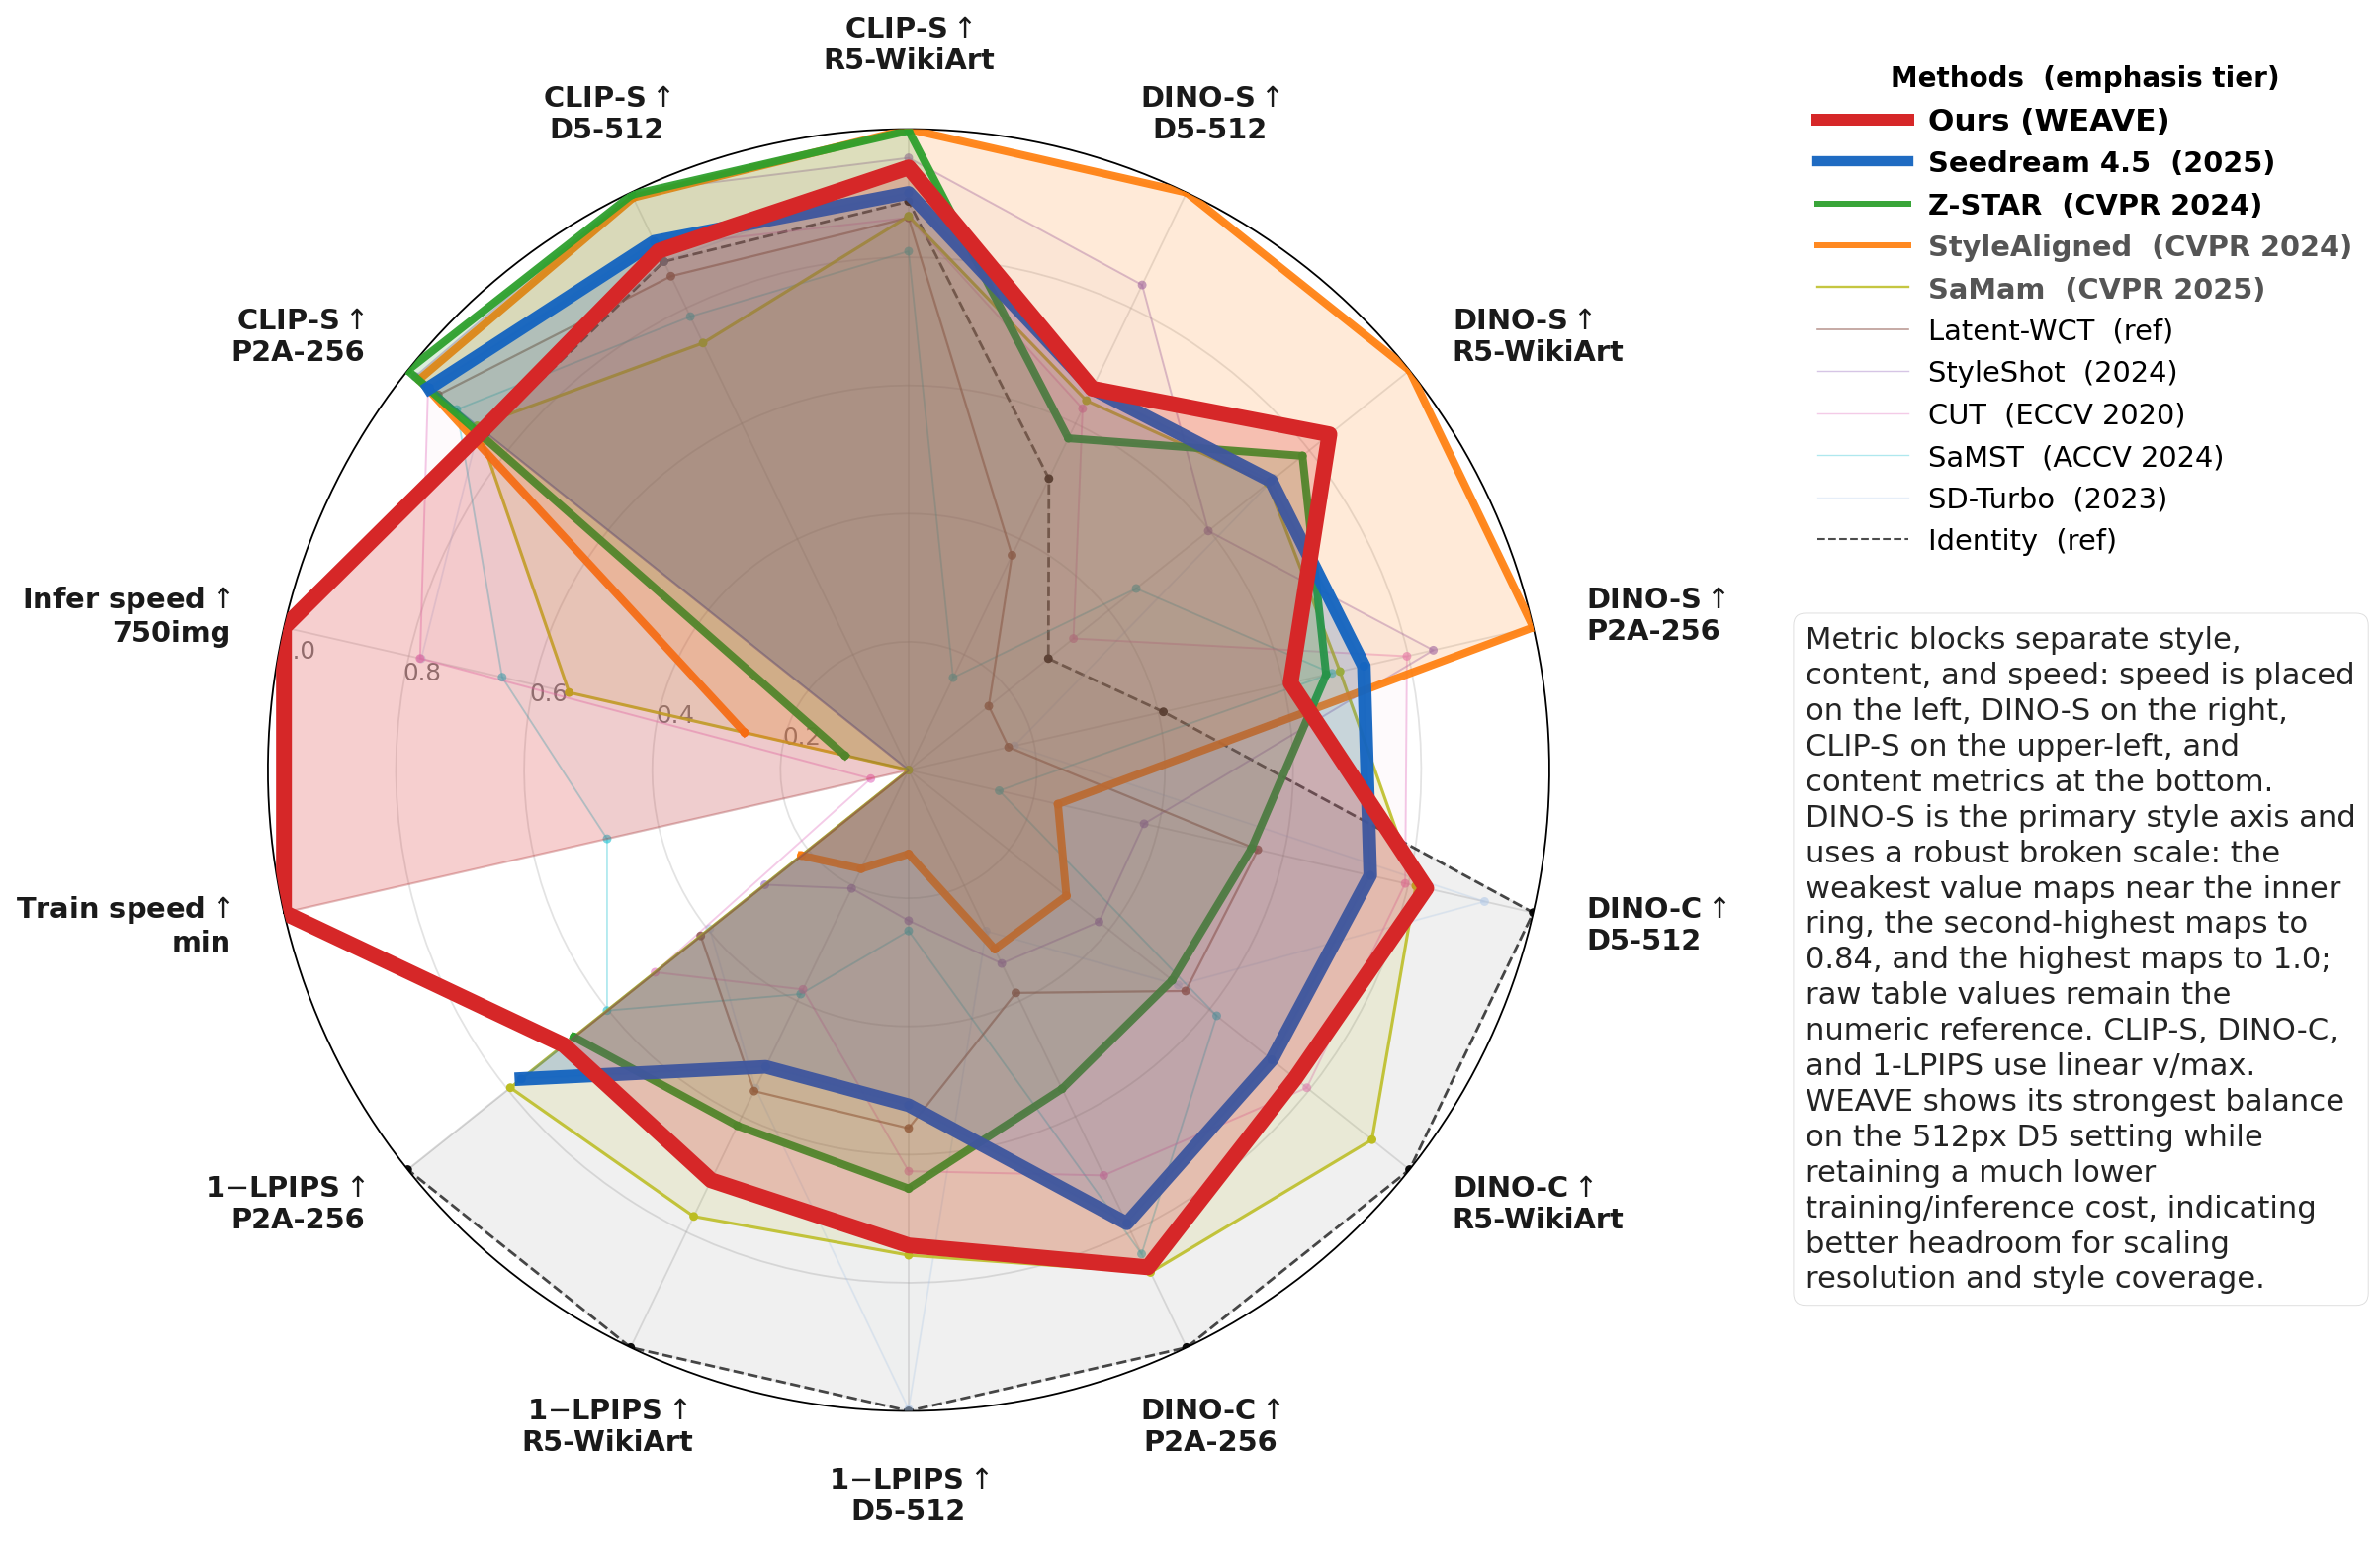
\includegraphics[width=0.9\linewidth]{radar_metric_blocks_A_clip_dinos_robustbreak.png}
\caption{Style, content, and cost across three benchmarks. DINO-S uses a broken visual scale to separate the middle tier; other axes are linearly normalized. Table~\ref{tab:main} gives raw values.}
\label{fig:radar}
\end{figure}
\paragraph{Reading the sandwich.}
The marks expose two operating regimes without changing the metrics: some rows remain
below IDT on style, while others cross TGT on content distance. Unmarked rows show that the
bracket is attainable by very different architectures. Its board dependence also motivates
computing IDT and TGT separately rather than using one absolute threshold.

\paragraph{D5 result.}
WEAVE records 0.486 DINO-S and 0.708 CLIP-S, above the corresponding IDT values of 0.419
and 0.693, while retaining 0.258 LPIPS and 0.829 DINO-C. Methods with higher DINO-S move farther from the source; Seedream
has nearly identical DINO-S but 0.477 LPIPS. Among trained rows above IDT on CLIP-S,
WEAVE has the lowest D5 LPIPS and the only sub-million-parameter network.

\paragraph{P2A and R5.}
WEAVE remains inside the bracket on P2A, although SaMam gives the best measured P2A
trade-off. On R5, WEAVE reaches the highest DINO-S among the trained lightweight methods
(0.523) with 0.290 LPIPS as the style space grows to 20 families.
Figure~\ref{fig:radar} summarizes the full profile.

\paragraph{Cost.}
WEAVE trains in 3 minutes on one RTX~3060 versus 39.5--436 minutes for the learned
baselines, and generates 750 images in 95\,s. Latent-WCT is faster but falls below IDT,
showing that analytic wavelet statistics alone do not replace learned transport.

\subsection{Mechanistic Ablations}
\label{sec:ablation}

Table~\ref{tab:ablation} compares variants from one five-epoch checkpoint. Removing AdaIN
or flow matching shifts the result toward source preservation, while removing cross-attention
changes every metric by at most 0.010. One Euler step and strong extrapolation degrade both
objectives, identifying the active paths and their stable operating range.

\begin{table}[ht]
\centering
\footnotesize
\setlength{\tabcolsep}{4pt}
\begin{tabular}{@{}lcccc@{}}
\toprule
Config & CLIP-S$\uparrow$ & LPIPS$\downarrow$ & DINO-S$\uparrow$ & DINO-C$\uparrow$ \\
\midrule
\textbf{Baseline} & \textbf{0.727} & \textbf{0.343} & \textbf{0.483} & \textbf{0.755} \\
\midrule
w/o AdaIN & 0.708 & 0.334 & 0.484 & 0.816 \\
w/o Flow Matching & 0.710 & 0.296 & 0.475 & 0.819 \\
w/o Cross-attention & 0.726 & 0.336 & 0.486 & 0.765 \\
\midrule
$\lambda_{LL}{=}0$ & 0.713 & 0.313 & 0.480 & 0.804 \\
lr $=5{\times}10^{-4}$ & 0.730 & 0.356 & 0.487 & 0.738 \\
\midrule
AdaIN $\alpha{=}0$ & 0.709 & 0.339 & 0.483 & 0.811 \\
AdaIN $\alpha{=}2.0$ & 0.717 & 0.297 & 0.485 & 0.802 \\
extrap $=1.0$ & 0.704 & 0.591 & 0.411 & 0.616 \\
num\_steps $=1$ & 0.709 & 0.476 & 0.376 & 0.448 \\
\bottomrule
\end{tabular}
\caption{Ablation on D5 (5 epochs, 750 pairs). The main result uses 10 epochs and a 0.3 LL target blend. Changes below 0.002 CLIP-S are omitted.}
\label{tab:ablation}
\end{table}

Setting $\lambda_{LL}=0$ moves the model toward the source, so weak LL supervision is useful
for coarse tone. Remaining low-impact sweeps are reported in the supplement.









\subsection{Generalization and Robustness}
\label{sec:gen}

\paragraph{Representation and adaptation.}
A matched RGB control performs worse on both style and content. Updating only the style
memory from 30 images clears IDT on eight held-out styles, with little gain from full
fine-tuning.

\paragraph{Unseen families.}
On five unseen WikiArt families, WEAVE gives the highest CLIP-S and DINO-C and the lowest
LPIPS (Table~\ref{tab:ooze}); SaMam is 0.015 higher on DINO-S but has higher LPIPS.
\begin{table}[ht]
\centering
\small
\resizebox{\linewidth}{!}{%
\begin{tabular}{@{}lcccc@{}}
\toprule
Method & CLIP-S $\uparrow$ & LPIPS $\downarrow$ & DINO-S $\uparrow$ & DINO-C $\uparrow$ \\
\midrule
Ours (WEAVE) & \textbf{0.7742} & \textbf{0.2802} & 0.5313 & \textbf{0.7587} \\
SaMam & 0.7577 & 0.3990 & \textbf{0.5466} & 0.7369 \\
SaMST & 0.7485 & 0.6213 & 0.3913 & 0.2680 \\
\bottomrule
\end{tabular}%
}
\caption{Zero-shot evaluation on Other5 (750 pairs) using the D5 checkpoint.}
\label{tab:ooze}
\end{table}

\paragraph{Basis and resolution.}
Daubechies-2 slightly improves CLIP-S but worsens LPIPS; Haar gives the better measured trade-off and has exact orthogonality with compact support. Native-resolution training also outperforms upsampling a low-resolution checkpoint, consistent with style information being carried by high-frequency bands that low-resolution training compresses.


\subsection{Plug-and-Play Extension to Pre-trained Diffusion Models}
\label{sec:plugin}

We add the same Haar and endpoint AdaIN operation to a frozen SD1.5 image-to-image pipeline without training. The base editor uses an empty prompt, strength 0.5, and 20 DDIM steps; the plugin aligns LH/HL/HH at scale 0.8 while leaving LL unchanged. On 600 off-diagonal D5 pairs, both CLIP-S and DINO-S increase ($p{<}10^{-15}$, paired $t$-test) with little content change, and the improvement remains on the full 750-pair board. The DWT--AdaIN--IDWT operation adds 4.9\,ms per image. This experiment tests transferability of the operator, not a claim that the small network and SD1.5 are otherwise equivalent.


\subsection{Mechanism Analysis}
\label{sec:mechanism}

\paragraph{Gradient spectrum.}
At $t{=}0.5$, the unweighted LL loss is $5{\times}$ larger than the high-frequency losses and its head gradient is $6{\times}$ larger. LL remains the largest input-gradient band after down-weighting, so the imbalance is not created solely by the chosen loss weights. This is evidence of frequency dominance in the trained system, although it does not by itself prove that every identity-like solution has the same cause.

\paragraph{Subband roles.}
Output probes show that LH/HL carry most of the measured style change, LL retains structure, and headless HH changes only through endpoint AdaIN. Inference-time module swaps agree: removing AdaIN sharply reduces the LH style-transfer ratio, while replacing it with full-covariance WCT adds content drift for little style gain. Together with the ablation table, these probes support the intended division of labor between learned transport and endpoint alignment.

\section{Discussion}
\label{sec:discussion}

The evidence supports a simple interpretation: flow matching moves the latent while preserving source structure, and endpoint AdaIN supplies the high-frequency style signal that the flow loss underweights. Neither component is sufficient alone (Table~\ref{tab:ablation}). Applying AdaIN at every Euler step would repeatedly pull statistics toward one reference and let that signal enter later velocity updates; applying it once keeps the learned trajectory and the analytic correction easier to separate.

\paragraph{What the evidence establishes.}
The argument is supported at three levels. First, the training probe measures a clear
low-frequency advantage in both loss and gradient norm. Second, the architecture assigns
LL and high-frequency corrections to separate coordinates and applies the image-specific
statistics update only at the endpoint. Third, interventions agree with these roles:
removing flow matching weakens transport, removing endpoint AdaIN weakens style movement,
and Latent-WCT does not clear IDT. Together, the evidence supports frequency dominance as
an important driver of the observed identity shortcut in this system. It does not claim
that frequency dominance is the only cause of identity behavior in every architecture.

\paragraph{Why a compact model is sufficient here.}
WEAVE does not learn image generation from scratch. The frozen VAE supplies a regularized latent space, the Haar transform fixes the coordinate system, and AdaIN performs a closed-form endpoint correction. The 903K network is responsible only for the residual transport that remains. This division explains why parameter count and training time can be small without treating the analytic components as learned capacity. It also explains the plugin result: the same endpoint operator improves a frozen SD1.5 editor because the operator acts on latent statistics rather than on network-specific weights.

\paragraph{Scope of the evaluation guideline.}
The sandwich guideline should be read narrowly. IDT and TGT make existing scores easier to interpret, but they are not perceptual ground truth or formal bounds. A method can cross a reference because of a metric mismatch, and a flagged cell is a prompt for visual inspection rather than a verdict. The proposal is intentionally modest: report two cheap reference rows, preserve the original metrics, and make the desired direction explicit. Human preference studies and artifact-sensitive measures remain complementary.

\paragraph{Limitations.}
WEAVE is domain-conditional rather than reference-image conditional. D5 contains only five deliberately separated styles, partly addressed by R5 and Other5. Protecting LL also makes palette-dominated styles harder, and one Haar level may miss cues that span several scales. The mechanism probes use one checkpoint family and automatic metrics; broader human evaluation is needed before extending the causal claim beyond this setting.

\section{Conclusion}

Style transfer should demonstrate both movement toward the requested style and retention of the source. We therefore advocate the IDT--TGT sandwich as a simple addition to standard evaluation: IDT shows what the metrics award to doing nothing, and TGT shows what they award to returning a source-independent target-style image. The two rows do not replace DINO, CLIP, or LPIPS; they give those scores a direction and an interpretable reference range. The marked cells in Table~\ref{tab:main} make this reading explicit while remaining local to each benchmark and metric.

WEAVE addresses the corresponding optimization problem by changing coordinates. A Haar
transform separates the dominant LL structure from high-frequency texture. A compact
rectified-flow network learns the content-aligned transport, while endpoint AdaIN moves
high-frequency statistics toward the requested style exactly once. Gradient, subband, and
module-swap probes show that the trained system follows this division of labor.

Across D5, P2A, R5, and five unseen families, WEAVE provides a stable content-preserving operating point rather than winning every metric. It uses 903K trainable parameters, trains in 3 minutes on one RTX~3060, and generates the 750-image board in 95 seconds. Applying the same endpoint operation to frozen SD1.5 improves style scores without retraining, suggesting that frequency-routed endpoint alignment is useful beyond the compact model. The remaining questions are equally clear: reference-image conditioning, multi-scale style cues, and human preference evaluation require further study.

\section*{Ethics Statement}
Style transfer tools can be misused to produce deceptive images or to misattribute stylistic authorship.
Our method operates at the domain level (e.g., ``Impressionism'') rather than the per-artist level.
This reduces the risk of imitating a specific living artist.
We do not condition on individual reference paintings.
The dataset is sourced from WikiArt and contains historically significant artworks.
It does not contain personal data.
We encourage downstream users to disclose when an image has been style-transferred and to respect source-content licensing terms.

\section*{Reproducibility Statement}
All experiments use public data (WikiArt) and a public VAE (Stable Diffusion v1.5 EMA VAE).
The experiments section gives the training configuration, hyperparameters, and evaluation protocol.
Training takes 3 minutes on a single RTX 3060 (12\,GB; 10-epoch wall-clock, batch 96).
Generation-only inference for 750 pairs needs about 95 seconds (8-step ODE + VAE decode; $\approx$71\,ms network generation and $\approx$52\,ms decode per image), and a full metrics pass (CLIP/LPIPS on top of generation) is about 2 minutes.
The 903K trainable parameter backbone checkpoint is 3.5\,MB.
We will release the code, the checkpoint, and the 750-pair evaluation protocol upon publication.

\bibliography{refs}

\end{document}
